\subsection{How are roads funded in Ohio?}

Roads in Ohio are funded through a combination of federal, state, and local sources. A significant portion of road funding provided by federal and state governments comes from gas taxes, which are currently set at $\$0.18$ per gallon for federal tax and $\$0.38$ per gallon for Ohio state tax. Additional sources for these 2 levels of government include vehicle registration fees, license plate fees, tolls, and driver's license fees. Funding for local governments largely comes from property taxes. Below, we provide an overview of road funding in Ohio from national, state, and local sources.

{\bf Federal Funding.} U.S Department of Transportation (USDOT) provides funding for road infrastructure through the Federal Highway Administration (FHWA). The FHWA provides funding for the construction, maintenance, and operation of highways, bridges, and tunnels. The federal government provides funding for road infrastructure through the Highway Trust Fund (HTF), which is funded by the federal gas tax. The HTF is divided into two accounts: the Highway Account and the Mass Transit Account. The Highway Account is used to fund highway construction and maintenance, while the Mass Transit Account is used to fund public transportation projects. The federal government also provides funding for road infrastructure through the Surface Transportation Block Grant Program (STBG) or Bipartisan Infrastructure Law \citep{USDOT_BIL_Ohio}, which provides funding for road projects that are not eligible for funding through the HTF. Nevertheless, federal government funding for road infrastructure is generally limited, as in 2022, about 4/5$^\text{th}$ of the funding came from state and local governments \citep{pgpf_htf_explained}.

{\bf State Funding.}
In Ohio, gas taxes, licensing fees and user fees account for $69\%$ of the state's road funding \citep{boesen2021}. The Ohio Department of Transportation (ODOT) is responsible for the allocation of state funds, which are used for both maintenance and new construction. However, about 70\% of funds go to new highway construction, 2\% is given to local governments as grants and only 4\% of state funds is directed towards road maintenance \citep{odot2023}. The remaining funds are part of payroll \& operating expenses, and other miscellaneous expenses. Hence, most of the road maintenance funding for local, neighborhood-specific roads in Ohio comes from local governments.


{\bf Local Funding.} Local governments in Ohio fund roads mainly through property taxes, although the extent of this funding varies across different localities. These municipalities have the authority to levy property taxes specifically for road maintenance, providing a crucial source of funding for the upkeep of local infrastructure. For instance, as per our correspondance with the Beavercreek Township, 61\% of their road funds come from property taxes, and only 8\% from gas taxes. Moreover, 77\% of funding for roads in Beavercreek township is provided by the local government and 11\% of overall local government budget is allocated to roadway maintenance \citep{schroeder2025}. We can see that these local roads are primarily funded by local governments in Ohio and road maintenance funding is a significant part of the local government's budget.


\subsection{Local Taxation in Ohio}

{\bf Background.} Ohio consists of 88 counties, each covering about 464 miles$^2$ (1,200 kilometers$^2$). Each county was historically divided into about 15 equally-sized townships, which do not cross county lines. Citizens can petition to incorporate as a village, which has a different type of government structure than a township and the ability to levy both income and property taxes, whereas townships may only levy property taxes. When a village exceeds 5,000 population in Ohio, it is reclassified as a city. Villages and cities may cross township and county lines, dissolve, or annex parts of contiguous townships. Villages, cities and townships, which we call “cities” for brevity, are the most local governmental unit in Ohio. Each local government covers about 18.2 miles$^2$ (47.1 km$^2$) on average. The Ohio Revised Code lets local governments collect a small amount of tax without a vote. Beyond this limited amount local governments put tax levies on the ballot to ask for additional money from voters. Ohio has 3,939 local governments in total as of 2022 \citep{stlouisfed2024local}.  

The type of tax levy we study is for the renewal of road tax levy, which covers a broad range of activities. Most of the renewal taxes we consider have stated purposes of “road and bridges repair”, “road repair”, “street fund”, and “street improvements”, although there are less common stated purposes like “repair and maintenance of streets and sewers system” and “resurfacing and rehabilitation of city streets.”  The construction of new roads and bridges, in contrast, would be funded with a tax levy for additional money, not a renewal tax; and it would likely be funded by a bond levy lasting 20 or 30 years.  We eliminate from our dataset stated purposes that might suggest new road construction like a 30-year 1.9-mill new tax in Moscow Village for “permanent improvements” and 0.5-mill new tax for 20 years in Shawnee Hills Village for “general construction and road and bridges repair.” Our dataset includes tax levies such as a 2-mill, 5-year renewal in Adams Township (Champaign County) in 1995; a 3-mill, 5-year renewal in Lore City Village in 2016; and a 2.5-mill, 5-year renewal in Pataskala City in 2007.

\noindent Levies that had originally passed typically expire, and the most common duration to collect a levy is five years, representing about 90\% of the road tax levies in our sample.  If a tax levy is renewed, taxes and funding continue.  If 50\% or fewer votes approve the levy, it fails.  When a tax levy for additional funding fails, there is no increase in funding, but existing funding from other tax levies continues as normal.  When a renewal tax levy fails, funding from that tax levy stops.  99\% of the road tax levies in our sample are property taxes and 1\% are income taxes.

{\bf Renewal levies.} Most regression discontinuity studies that use voting data to look at the impact of funding changes examine new tax levies for additional funding.  \cite{cellini2010value} observes that votes for additional tax money may not be statistically independent; a vote may be proposed until it passes.  We minimize this source of endogeneity of new votes by only considering renewal votes \citep{brasington2017school}.  While a government may choose when to put a vote for additional funding on the ballot and keep proposing the new tax until it is passed, when a vote passes it has an expiration date.  So if a road tax levy for additional funding passes in 2007 to last five years, in 2012 voters will have the chance to renew or reject the tax.  The timing of the vote in 2012 is not endogenous, having been set in 2007.  If voters renew it in 2012, it will be up for renewal again in 2017. 

{\bf Spending impact of failing to renew a levy.} When a renewal tax levy fails, the local government loses the funding from that tax levy. The local government may still have tax levies for other purposes in effect, but the road tax levy that failed to renew is no longer collected. To investigate the amount of loss in road maintenance funds after a failure to renew road tax levy, we use information from the levy database, along with home prices and demographics information. We use these data to determine the dollar amount in consideration when a household is making a decision on whether to vote for or against a renewal road tax levy, and we call it Average Road Tax per household, which is the tax amount that a household will be paying if the levy is successfully renewed. Average Road Tax per household is computed using the following formula -

\begin{equation}
\text{Average Road Tax per household}_{it} = \text{millage rate}_{it} \times \text{Average Assessed value}_{it}
\end{equation}

where $i$ is the city, $t$ is the year, and millage rate \footnote{Millage is property tax rate expressed in mills (tax per \$1000 of assessed value)} is the predetermined millage amount set for the road tax levy. The average assessed value is 35\% of the average appraisal value\footnote{Assessment ratio of 35\%, as set by \cite{OhioRealPropertyTax}}, which for our study equals the average sale price of homes in the city for that year. From this, we can also compute the average road tax per city by multiplying the average road tax per household with the number of households in the city.

Although we acknowledge large variation in the appraisal value across neighborhoods and in millage rates across referendums, we find that the average road tax per household is \$76, and the average road tax per city is \$167,011 as shown in Table \ref{tab:levy_stats}. We do not observe any significant difference in the average road tax per household between cities that renew and cut road tax levies, which suggests the levies up for renewal were not systematically different between areas that renewed and areas that failed to renew them. Whenever a renewal tax levy fails, the local government loses the funding from that tax levy, which is the average road tax per city. This loss in funding directly impacts local government's spending budget needed to maintain local roads in Ohio.

% This average road tax accounts for 15\% of a local government's budget for road maintenance.

\begin{table}[ht]
    \centering
    \caption{Spending impact of failing to renew a Road Tax Levy}
    \label{tab:levy_stats}
    \begin{threeparttable}
    \begin{tabular}{p{5cm}ccc}
    \hline\hline
    & \textbf{Aggregate} & \textbf{Renewed} & \textbf{Cut} \\
    \hline
    \textbf{Panel A: road tax per household and city} \\
    Mean & 76 & 75 & 79 \\
       & (55) & (53) & (62) \\
    \hline
    \textbf{Panel B: road tax per city} \\
    Mean & 167,011 & 167,648 & 163,547 \\
       & (340,268) & (340,628) & (338,671) \\
    \hline\hline
    \end{tabular}
    \begin{tablenotes}[flushleft]
      \footnotesize
      \item \textit{Notes:} 
      This table presents descriptive statistics for two measures of the money collected via road tax levies. 
      \textbf{Panel A} reports the mean and standard deviation (SD) of the road tax per household per year. 
      \textbf{Panel B} reports the mean and SD of the total road tax collected per city. 
      “Aggregate” denotes the full sample, while “Renewed” and “Cut” refer to levies that were renewed and failed to renew respectively.
      All monetary values are in constant 2010 U.S. dollars and rounded to the nearest integer.
    \end{tablenotes}
    \end{threeparttable}
\end{table}




% We also sample financial audits of cities in our sample whose renewal tax levies fail.  

\subsection{Tax Cuts \& Evidence of Road Quality} \label{sec:road_quality}

To understand the effect of cutting local road tax on road quality, we fine-tune a Vision Transformer (ViT) model, gpt-4o by OpenAI, on satellite imagery data from \cite{brewer2021}. Following the seminal work on text-based Transformers in Natural Language Processing (NLP) by \cite{vaswani2017attention}, ViTs were introduced by Google Brain's team and are part of a recent class of deep learning models that have shown to outperform Convolutional Neural Networks (CNNs) on image classification tasks \citep{dosovitskiy2020image}. Below, we outline the steps we take to assess road quality using the ViT model.


% We use the ViT model to classify road images into three categories: good, average, and poor. We then use the classification results to assess the quality of roads in different neighborhoods in Ohio. We collect road images for areas that were within the average effective RD bandwidth provided in Table \ref{tab:median_sale_amount} and ensure that we have pre and post referendum images for both, the treatment and control groups. This allows us to construct a novel database of road images and assess the impact of cutting local road tax on road quality.

{\bf Satellite Images for fine-tuning.} In order to enable ViTs to accurately predict road quality, we needed large-scale road-image data to fine-tune OpenAI's gpt-4o, a Large Language Model (LLM) with multi-modal ability that has shown to outperform various other models and benchmarks \citep{achiam2023gpt}. We use the road-image dataset by \cite{brewer2021} which consists of 53,677 labeled images of road infrastructure across the United States. The dataset includes images of roads in different conditions, and a classification representing quality of the road: 0 (poor), 1 (decent) and 2 (high). 

{\bf Ohio Satellite Images.} We use satellite images from Google Earth Pro for roads in different neighborhoods in Ohio. We collect road images for areas that were within the average effective RD bandwidth provided in Table \ref{tab:median_sale_amount} and ensure that we have pre and post referendum images for both, the treatment and control groups. This allows us to construct a novel database of road images, which we use to classify road quality for areas that were part of our quasi-experiment. Figure \ref{fig:road_quality_examples} presents 2 examples of road images from Ohio, one from a road that was classified as high and the other as poor quality.

\begin{figure}[ht]
    \centering
    \begin{minipage}{0.59\textwidth}
        \centering
        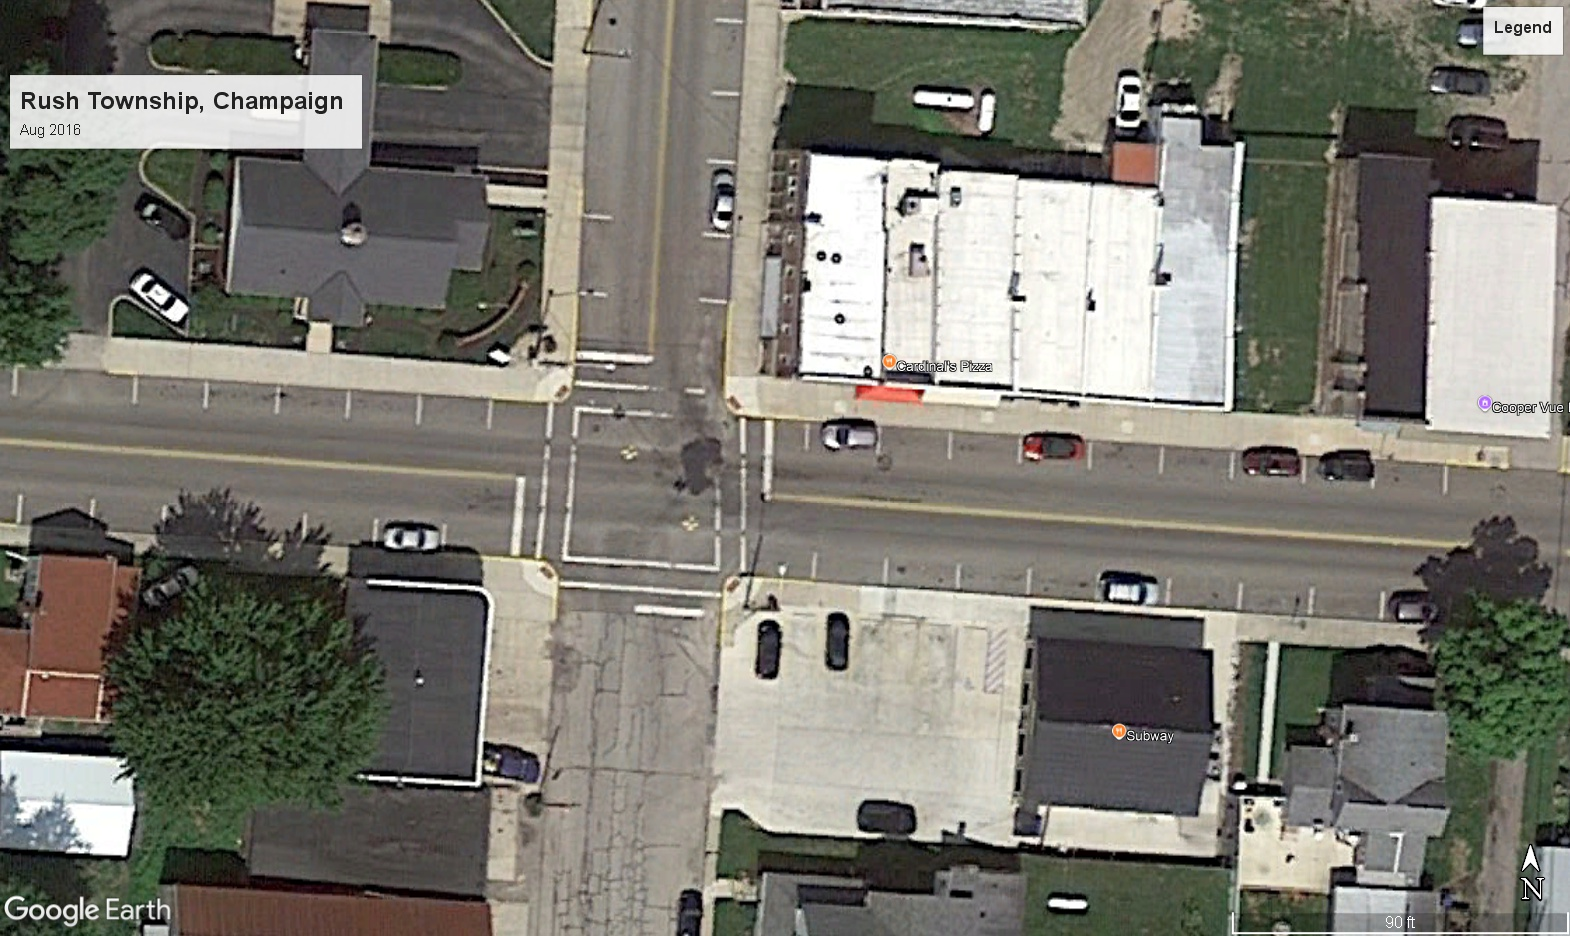
\includegraphics[width=\textwidth]{images/rush_twp_champaign_aug16.jpg}
        \caption*{(A) A {\bf \underline{Poor}} Quality Road}
    \end{minipage}
    \hspace{0.5in}
    \begin{minipage}{0.59\textwidth}
        \centering
        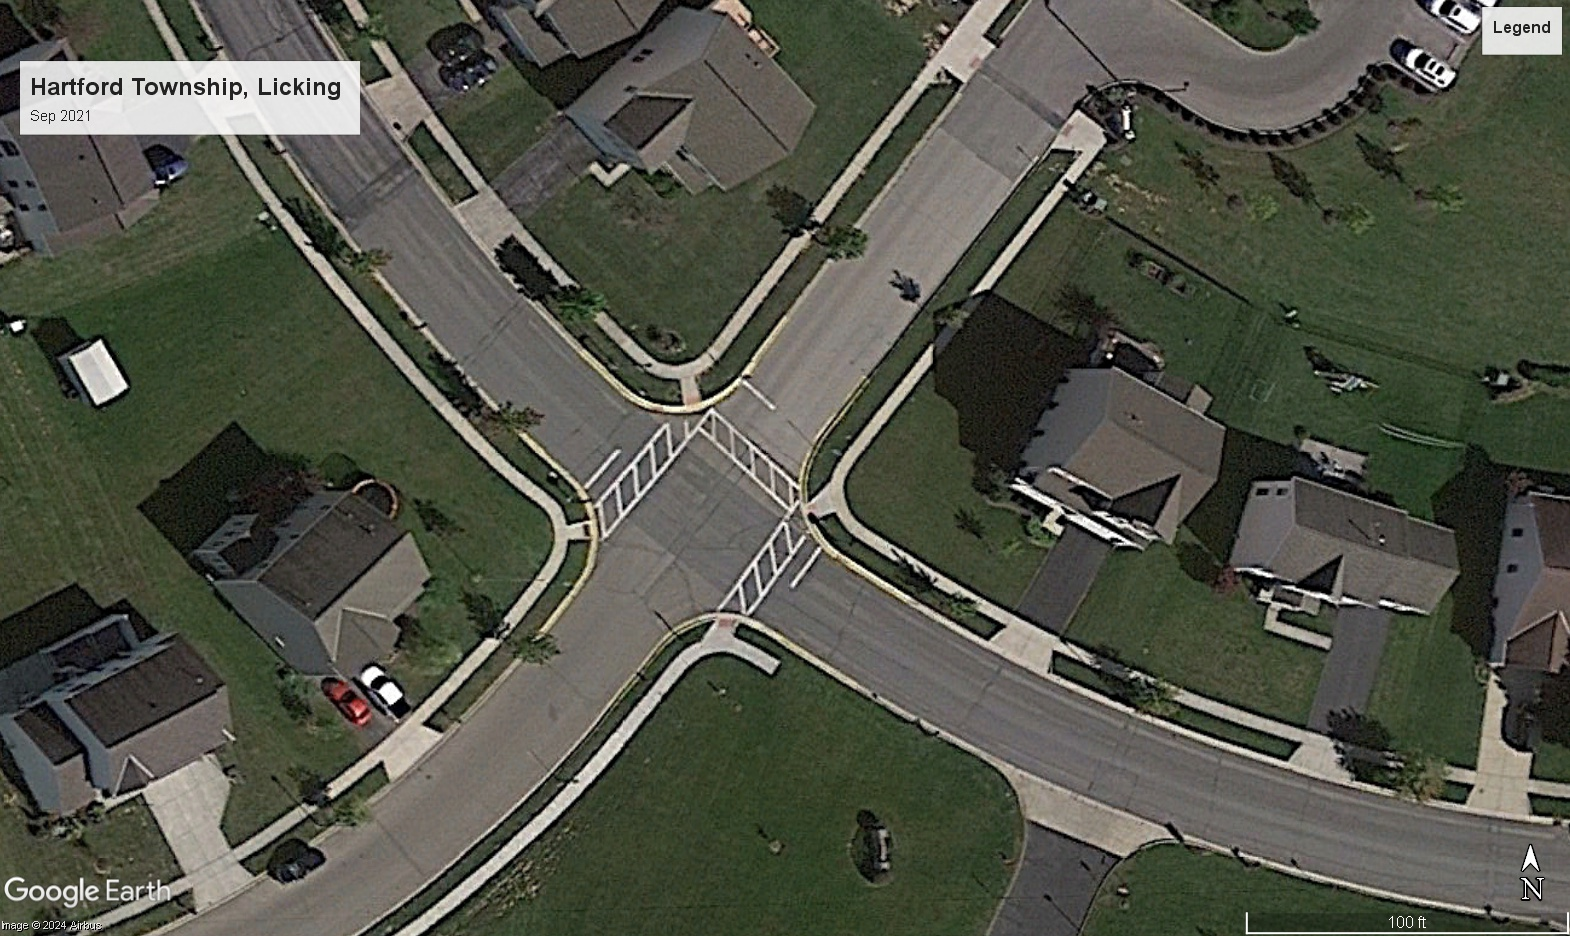
\includegraphics[width=\textwidth]{images/hartford_twp_licking_sep21.jpg}
        \caption*{(B) A {\bf \underline{High}} Quality Road}
    \end{minipage}
    \caption{Road Quality Satellite images for Ohio}
    \label{fig:road_quality_examples}
\end{figure}

{\bf Fine-tuning process.} Fine-tuning a ViT involves taking a pretrained model and adapting it for specific image-classification task. We fine-tune gpt-4o, a pretrained model with over 200 billion parameters, on the road-image dataset by \cite{brewer2021} to classify road images into three categories: 0, 1 and 2. Next, we divide the data into traning and validation datasets. Using OpenAI's API, we set up a training seed, convert the images into their corresponding base64 encoding and fine-tune the model on the road-image dataset for 10 epochs with a batch size of 9 and a learning rate multiplier of 2. In section \ref{sec:road_quality_decline}, we present the results from our fine-tuned model, when applied on roads in areas with close elections within our effective bandwidth. For full details on the modeling methodology, fine-tuning results and robustness tests, see \cite{2025predicting}. 

% We use the classification results to assess the quality of roads in different neighborhoods in Ohio. We collect road images for areas that were within the average effective RD bandwidth provided in Table \ref{tab:median_sale_amount} and ensure that we have pre and post referendum images for both, the treatment and control groups. This allows us to construct a novel database of road images and assess the impact of cutting local road tax on road quality.

% {\bf Predicting Road Quality.} 




% \bf{Analyzing satellite images.} Following \cite{brewer2021}

% \bf{Street Images.} We utilize a 

% \clearpage

% \subsection{Road Maintenance Funding}



\subsection{Running Variable}

The running variable plays a critical role in regression discontinuity, which in this study represents the proportion of votes against the renewal of a road tax levy. 

A vote share of more than 50 means the renewal road tax levy fails and tax will no longer be collected, resulting in a stoppage of road funding via that particular tax levy. However, other road tax levies may continue to be in effect, and funds from current expense tax levies may still be used for road maintenance. There are 3,184 referendum results in our sample, 83\% of which renew the tax, and 17\% of which cut taxes and road maintenance. We quantify the size of the cut in road spending a city faces in two ways. The Great Financial Crisis falls in the middle of our dataset, so readers might wonder if voting behavior was affected, but we find vote share the same to two decimal points during and outside the years 2008-2009. 

Our key identification assumption is that the election results are not predetermined and vote share is not precisely manipulated to fall just above or below the cutoff. This asumption allows use to exploit the randomization around the cutoff and provides the variation needed to identify the causal effect of cutting road tax. We test this assumption using a density test detailed below and covariate balance tests (see Appendix \ref{sec:appxb}).

{\bf Density test.} Classic regression discontinuity design (RDD) assumption states that agents cannot precisely manipulate the running variable to fall just above or below the cutoff. In our context, it means that the election results are not determined prior to when the ballot takes place. In other words, no individuals, organizations, higher levels of government, foreign governments, or the firm that programs the voting machines are dictating the precise vote share for the renewal road tax levy referendums raised by a city. The standard way to test this assumption is to perform a density test like that of \cite{cattaneo2020simple}, which is based on the idea that manipulation of elections might cause a clustering of votes just to one side of the cutoff, with a pronounced drop-off on the other side of the cutoff. The $p$-value of this density test is 0.98. A histogram of vote share is shown in Figure \ref{fig:running_var_hist} that graphically illustrates the lack of abrupt change in density.

\begin{figure}[ht]
    \centering
    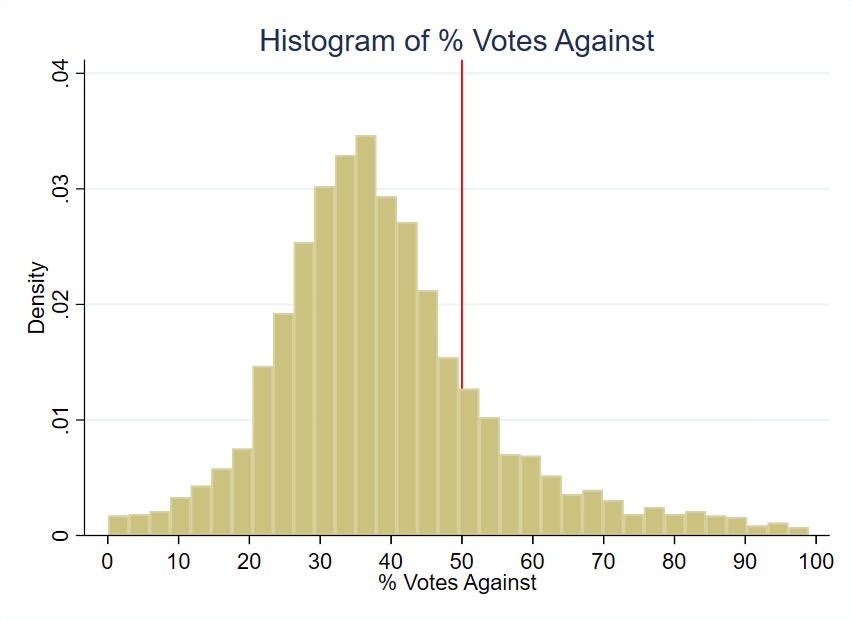
\includegraphics[width=\textwidth,keepaspectratio]{images/votes_pct_against_histogram.png}
    \caption{Histogram of Running Variable}
    \label{fig:running_var_hist}
\end{figure}

Although Table \ref{tab:variable_means_sd} shows covariate balance between sets of cities that pass and fail to renew road tax levies, covariate values could still jump from one side of the cutoff to another. A drop in education levels, for example, could cause a drop in house prices that might coincide with a change in treatment, so that what might look like a treatment effect from cutting taxes and spending might in fact be caused by lower education levels. Graphs of covariate smoothness around the cutoff are found in the Appendix \ref{sec:appxb}. A formal way to assess covariate smoothness is to use each covariate as an outcome variable in a regression of the running variable and a treatment effect dummy. When we do so, the $p$-value of the treatment effect dummy varies from 0.13 to 0.98, indicating no statistically significant jump in covariate values. 

\subsection{Outcome Variables}

{\bf Median Housing Prices.} Our house price data comes from a CoreLogic® dataset of actual sales transaction prices in Ohio from 1995 through 2021 containing over 7 million observations. The dependent variable, \textit{Median House Price}, reflects the median sale price of houses within a specific city and year. For example, for the houses sold in Delaware Township during the year 2002, the median sale price was \$205,041. We take precaution to only include arm’s-length transactions, and we restrict our attention to single-family residential structures for comparability.  The overall sample mean for the 10-year period from the time of vote considered in this study is \$166,082 in constant 2010 dollars with a standard deviation of \$372,135 which suggests presence of some outliers. Although our use of median sale price addresses outliers, one of our robustness checks drops 1\% tails and re-estimates the treatment effects.  The mean for this winsorized sample is \$150,375 in constant 2010 dollars with a standard deviation of \$116,020. 

\begin{figure}[ht]
    \centering
    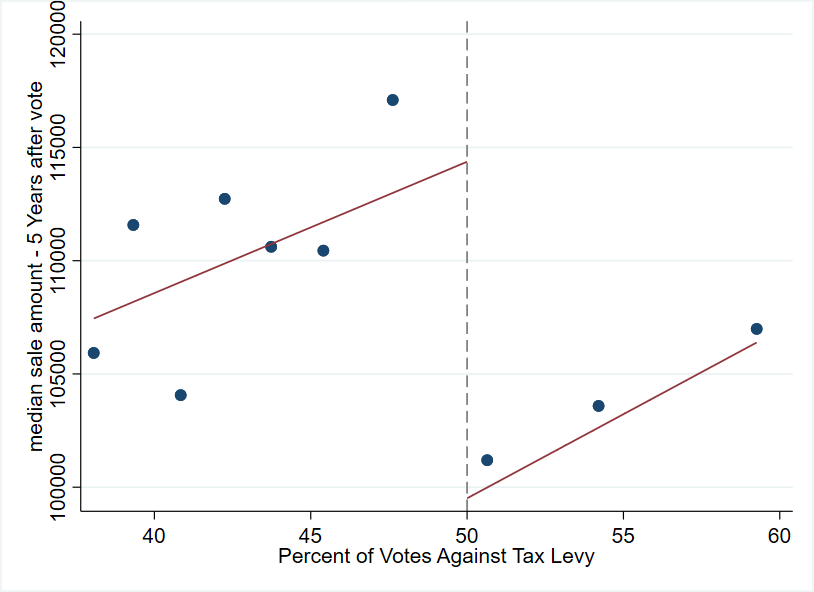
\includegraphics[width=0.8\textwidth,keepaspectratio]{images/rd_plot_year_5_after_vote.png}
    \caption{Median Sale Price of Homes: 5 years after vote}
    \label{fig:hp_year5_after}
\end{figure}

Figure \ref{fig:hp_year5_after} shows house prices from 5 years after the vote graphed against the percent of votes for the tax levy. The points represent the mean house price for the 10 representative bins of vote shares for the average effective bandwidth around the cutoff of 50\%. The graph shows a clear discontinuity in house prices at the cutoff, which is the basis for our identification strategy. We observe a sharp decline after the cutoff in house prices, indicating that the failure to renew a road tax levy has a negative impact on house prices.


\subsection{Covariates}

Covariates can be useful in regression discontinuity studies, although they are not necessary for the identification of treatment effects.  One use of covariates is to increase the precision of treatment effect estimates.  The other is to see if cities that barely pass and fail tax levies are similar to each other like the theory of regression discontinuity says they should be. Table \ref{tab:variable_means_sd} shows covariate means for both the global sample of all votes in the data set as well as the local sample within a representative effective bandwidth of the 0.50 cutoff. The effective bandwidth displayed in Table \ref{tab:variable_means_sd} is the mean bandwidth for all the housing outcome regressions. The first columns for the global sample show similar values of characteristics between cities that renew and cut road taxes and spending, but it is the two rightmost columns that are critical for the credibility of the regression discontinuity design.   

Table \ref{tab:variable_means_sd} demonstrates the covariate balance between cities that renew their tax levies and those that do not, indicating similar demographic and economic profiles across both groups. The data, captured at the time of the vote, shows minimal differences within the effective bandwidth: the mean population differs by only 301, and median family income varies by \$436, measured in 2010 U.S. dollars. Other variables, including poverty rates, married household percentages, educational attainment, age distribution, and racial composition, show differences of two percentage point or less, bolstering the comparability of the two groups.

\begin{longtable}{p{4cm}cccccc}
    \caption{Variable Means \& Standard Deviation by Tax Levy Renewal Status} \label{tab:variable_means_sd} \\
    \hline
    Variable & \multicolumn{3}{c}{Global} & \multicolumn{2}{c}{Effective} \\
    \cmidrule(lr){2-4} \cmidrule(lr){5-6}
    & Full Sample & Renewed & Cut & Renewed (Control) & Cut (Treatment) \\
    \hline
    \endfirsthead

    \multicolumn{6}{c}{{\bfseries \tablename\ \thetable{} -- continued from previous page}} \\
    \hline
    Variable & \multicolumn{3}{c}{Global} & \multicolumn{2}{c}{Effective} \\
    \cmidrule(lr){2-4} \cmidrule(lr){5-6}
    & Full Sample & Renewed & Cut & Renewed (Control) & Cut (Treatment) \\
    \hline
    \endhead

    \hline \multicolumn{6}{r}{{Continued on next page}} \\
    \endfoot

    \hline
    \endlastfoot

    %%%%%%%%%%%%%%%%%%%%%%%%%%%
    %%  Panel A (UPDATED)   %%
    %%%%%%%%%%%%%%%%%%%%%%%%%%%
    % \multicolumn{6}{l}{\textbf{Panel A. Covariates}} \\
    Population & 5,072 & 4,733 & 5,139 & 4,885 & 5,186 \\
                & (7,936) & (7,291) & (8,058) & (7,036) & (8,229) \\
    Poverty Rate & 0.11 & 0.11 & 0.11 & 0.10 & 0.11 \\
                    & (0.08) & (0.07) & (0.08) & (0.07) & (0.08) \\
    \% with Kids & 0.39 & 0.40 & 0.39 & 0.39 & 0.39 \\
                    & (0.08) & (0.08) & (0.08) & (0.07) & (0.08) \\
    \% Households with Children under 18 & 0.09 & 0.09 & 0.09 & 0.09 & 0.08 \\[-2.3em]
                                            & (0.06) & (0.05) & (0.06) & (0.06) & (0.05) \\
    \% Less than High School Education & 0.16 & 0.18 & 0.15 & 0.18 & 0.16 \\[-2.3em]
                                        & (0.11) & (0.12) & (0.11) & (0.12) & (0.10) \\
    \% Some College Education & 0.25 & 0.24 & 0.25 & 0.24 & 0.25 \\[-2.3em]
                                & (0.06) & (0.06) & (0.06) & (0.07) & (0.06) \\
    \% Renters & 0.20 & 0.20 & 0.20 & 0.19 & 0.20 \\
                & (0.11) & (0.10) & (0.11) & (0.09) & (0.11) \\
    Unemployment Rate & 0.05 & 0.05 & 0.05 & 0.05 & 0.06 \\
                            & (0.04) & (0.03) & (0.04) & (0.03) & (0.04) \\
    \% White & 0.96 & 0.97 & 0.96 & 0.97 & 0.97 \\
                & (0.07) & (0.07) & (0.07) & (0.07) & (0.08) \\
    \% Black & 0.02 & 0.02 & 0.02 & 0.02 & 0.02 \\
                & (0.07) & (0.06) & (0.07) & (0.07) & (0.07) \\
    \% Married & 0.59 & 0.60 & 0.59 & 0.61 & 0.60 \\
                & (0.09) & (0.08) & (0.09) & (0.08) & (0.09) \\
    \% Separated & 0.01 & 0.01 & 0.01 & 0.01 & 0.01 \\
                    & (0.01) & (0.01) & (0.01) & (0.01) & (0.01) \\
    Income Heterogeneity Index & 0.10 & 0.09 & 0.10 & 0.09 & 0.09 \\[-2.3em]
                                & (0.08) & (0.07) & (0.08) & (0.07) & (0.06) \\
    Median Family Income & 61,018 & 58,761 & 61,467 & 59,934 & 60,370 \\[-2.3em]
                            & (17,649) & (13,915) & (18,270) & (13,655) & (15,713) \\
    \% Under 5 Years Old & 0.06 & 0.06 & 0.06 & 0.06 & 0.06 \\
                            & (0.02) & (0.02) & (0.02) & (0.02) & (0.02) \\
    \% Aged 5 to 17 & 0.20 & 0.21 & 0.20 & 0.20 & 0.20 \\
                    & (0.05) & (0.04) & (0.05) & (0.04) & (0.05) \\
    \% Aged 18 to 64 & 0.60 & 0.60 & 0.60 & 0.60 & 0.60 \\
                        & (0.05) & (0.05) & (0.05) & (0.04) & (0.05) \\
    \% Racial Minority & 0.04 & 0.03 & 0.04 & 0.03 & 0.03 \\
                        & (0.07) & (0.07) & (0.07) & (0.08) & (0.07) \\
    Number of Observations & 3,184 & 2,656 & 528 & 653 & 269 \\

\end{longtable}


% \begin{tablenotes}
%     \small
%     \item Notes: Panel A shows covariates used in estimating the treatment effect of failing to renew a road tax levy. Covariate means at the time of the vote are shown along with standard deviations in parentheses. The unit of observation is city-year. 'Income' is median family income in constant 2010 U.S. dollars. 'Global' refers to the full sample of city-year votes; 'Effective' refers to city-year votes within the mean estimated optimal bandwidth of 10 percentage points around the cutoff for years 1995 through 2021. The treatment group reflects cutting road funding by failing to renew the road tax levy. The control group reflects maintaining road funding by renewing the road tax levy. Panel B shows means of outcome variables for placebo years t - 3, t - 2, and t - 1.
% \end{tablenotes}


Table \ref{tab:variable_means_sd} shows that the treatment and control groups are well-balanced with respect to the covariates considered, suggesting that the groups are comparable and any observed differences in outcomes can more confidently be attributed to the treatment effect rather than to pre-existing differences.

